%\documentclass[preprint,12pt]{elsarticle}
\documentclass[final,3p,times,onecolumn]{elsarticle}
%\documentclass[preprint,5p,times]{elsarticle}
%\documentclass[preprint,12pt]{elsarticle}

\usepackage{amssymb}
\usepackage{makecell}
\usepackage{multirow}
\usepackage{booktabs}
\usepackage{multirow}
\usepackage{soul}
\usepackage{graphicx}
\usepackage{lscape}
\usepackage{subcaption}
\usepackage{booktabs}
\usepackage[T1]{fontenc}
\usepackage[utf8]{inputenc}
%\usepackage{lmodern}
\usepackage[english]{babel}
\usepackage[colorlinks]{hyperref}
\usepackage{acronym} 
\usepackage{longtable}
\usepackage{threeparttable} % For table notes
\usepackage{array}          % For p{} column widths
\usepackage{caption}        % For better control of table captions
\captionsetup[table]{skip=10pt} % Adds some space between caption and table
%\input{glossary}
%\makeglossaries

%\newenvironment{framedglossary}%
%  {\begin{mdframed}}%
%  {\end{mdframed}}
%% The amsthm package provides extended theorem environments
%% \usepackage{amsthm}


%% The lineno packages adds line numbers. Start line numbering with
%% \begin{linenumbers}, end it with \end{linenumbers}. Or switch it on
%% for the whole article with \linenumbers.
%% \usepackage{lineno}

\journal{Energy Research \& Social Science }

\begin{document} 

\begin{frontmatter}

%% Title, authors and addresses

%% use the tnoteref command within \title for footnotes;
%% use the tnotetext command for theassociated footnote;
%% use the fnref command within \author or \address for footnotes;
%% use the fntext command for theassociated footnote;
%% use the corref command within \author for corresponding author footnotes;
%% use the cortext command for theassociated footnote;
%% use the ead command for the email address,
%% and the form \ead[url] for the home page:
%% \title{Title\tnoteref{label1}}
%% \tnotetext[label1]{}
%% \author{Name\corref{cor1}\fnref{label2}}
%% \ead{email address}
%% \ead[url]{home page}
%% \fntext[label2]{}
%% \cortext[cor1]{}
%% \affiliation{organization={},
%%             addressline={},
%%             city={},
%%             postcode={},
%%             state={},
%%             country={}}
%% \fntext[label3]{}

%Option 1 \title{Modeling Household Behavior in the Context of Solar Home System Electrification: A Case Study in Raqaypampa, Bolivia.}
%Option 2 \title{Energy, Culture, and Community: Understanding and Modeling Energy Behavior in Rural Raqaypampa, Bolivia}

\title{Modeling Household Behavior in the Context of Solar Home System Electrification: A Case Study in Raqaypampa, Bolivia.}

%% use optional labels to link authors explicitly to addresses:
%% \author[label1,label2]{}
%% \affiliation[label1]{organization={},
%%             addressline={},
%%             city={},
%%             postcode={},
%%             state={},
%%             country={}}
%%
%% \affiliation[label2]{organization={},
%%             addressline={},
%%             city={},
%%             postcode={},
%%             state={},
%%             country={}}

\author[inst1,inst2]{Claudia Sanchez-Solis}

\affiliation[inst1]{organization={Centro Universitario de Investigaciones en Energías, Universidad Mayor de San Simón},%Department and Organization
            %addressline={Address One}, 
            city={Cochabamba},
            %postcode={00000}, 
            %state={State One},
            country={Bolivia}}

\affiliation[inst2]{organization={Integrated \& Sustainable Energy Systems (ISES), Department of Mechanical and Aerospace Engineering, Université de Liège},%Department and Organization
            %addressline={Address Two}, 
            city={Liège},
            %postcode={22222}, 
            %state={State Two},
            country={Belgium}}

\affiliation[inst3]{organization={Instituto de Investigaciones en Ciencias Sociales, Universidad Mayor de San Simón},%Department and Organization
            %addressline={Address Two}, 
            city={Cochabamba},
            %postcode={22222}, 
            %state={State Two},
            country={Bolivia}}

\author[inst3]{Jaime Zambrana}
\author[inst1]{Sergio Balderrama}
\author[inst2]{Silvain Quoilin}
\begin{abstract}
%% Text of abstract

\end{abstract}

%%Graphical abstract
\begin{graphicalabstract}
%\includegraphics{grabs}
\end{graphicalabstract}

%%Research highlights
\begin{highlights}
\item Research highlight 1
\item Research highlight 2
\end{highlights}

\begin{keyword}
%% keywords here, in the form: keyword \sep keyword
Rural electrification \sep Solar Home Systems \sep Energy Culture \sep Developing countries \sep Energy Behavior \sep Energy Use

\end{keyword}

\end{frontmatter}

%% \linenumbers

%% main text
\section{Introduction}
\label{sec:sample1}

\begin{itemize}
    \item Set the scene: context and background (global energy use scenario, etc).
    Energy use around the world keeps evolving in time as a product of a broad range of factors that involve external conditions, technological advancements and personal decisions. Naturally, this evolution is heterogeneous and highly dependent on contexts. As a result, the energy consumption disparities persist
    \item Why to focus on energy use/energy behavior? Rural communities! Justify it
    Focus on energy demand drivers and evolution remains a crucial topic, specially if we think about the societal groups that fall out of the common energy consumption patterns. These can be rural settlements with different cultural backgrounds
    \item Literature review as a narrative of existing knowledge on energy behavior and energy culture.
    \item Identify the Gap
    Lack of social and human dimension?
    Interdisciplinary approaches
    Methodological challenges
    Using of sensors on research demonstrated bias ob self-reported energy use, with bigger gaps in specific situations, however, they are not enough by themselves when trying to understand behavior dynamics, they are a complement for surveys \cite{rom_using_2020}.
\subsection{Study Objectives and Structure}
\label{sec:objectives}

    \item Research question and objectives
    
    \hl{How do socioeconomic conditions, cultural norms, energy practices, and material factors influence energy behavior in rural Raqaypampa, Bolivia, and how can these insights improve the modeling of energy demand to support sustainable solutions planning?}
    Option 2: How do socio-economic conditions, cultural norms, and material realities shape energy behavior in an indigenous territory, and how can these insights be operationalized to support bottom-up energy demand modeling for inclusive electrification planning?
    
    The aim of this paper is to investigate how socioeconomic conditions, cultural norms, energy practices, and material factors shape energy behavior in rural communities. By exploring these dynamics, the study seeks to generate insights that can enhance the modeling of energy demand, ultimately contributing to the development of sustainable and context-sensitive energy solutions. A case study in Raqaypampa, Bolivia is considered.
    
    \item Brief description of the Approach and methodology
    \item Contributions and significance
    
    The key contributions of the paper are:
    \begin{itemize}
        \item A detailed empirical case study serves as the focal point, providing context-specific insights into energy behavior and its influencing factors in isolated indigenous communities, with broader applicability to similar settings worldwide.
        \item An extended mixed-methods analysis is applied within the Energy Cultures framework, offering a comprehensive approach to examining the relationships among diverse variables and presenting a holistic view of energy dynamics in a rural context.
        \item Empirical evidence contributes to the discourse on effective data collection methodologies in data-scarce settlements by exploring the interplay between self-reported energy practices and actual electricity consumption, using a modeling approach. These findings bridge gaps in demand data availability and improve the accuracy of energy behavior analyses in remote communities.
        \item Socio-cultural dimensions are integrated into a demand simulation approach, enhancing the precision and contextual relevance of modeling energy behavior in the study area.
    This paper contributes to advancing bottom-up energy modeling by embedding socio-cultural dimensions of energy behavior into the RAMP tool. Through empirical insights from rural Raqaypampa, we demonstrate how user practices, priorities, and constraints can reshape load profiles and challenge dominant modeling assumptions, offering a more grounded foundation for sufficiency-based planning.

    Contextualized empirical insights:
    This paper offers a detailed empirical case study of energy behavior in an isolated Indigenous community (Raqaypampa, Bolivia), uncovering the socio-cultural, economic, and material factors that shape energy practices. While rooted in a specific context, the findings offer transferable insights for similar underserved settings across the Global South.
    
    Innovative use of the Energy Cultures framework:
    By applying an extended mixed-methods approach within the Energy Cultures framework, the study advances a holistic analytical lens for capturing the interplay between norms, practices, and material culture in rural energy use — a methodological innovation rarely applied in energy modeling contexts.
    
    Bridging data gaps through modeling and fieldwork integration:
    The paper demonstrates how triangulating self-reported practices with modeled demand profiles enhances the reliability of energy behavior data in data-scarce environments. This contributes to the discourse on demand estimation methodologies for off-grid and low-consumption contexts.
    
    Modeling contribution: integrating socio-cultural dimensions into demand simulation:
    The study operationalizes qualitative and behavioral insights into the RAMP bottom-up model, illustrating how demand modeling can be made more context-sensitive. This contributes to the development of energy models that support sufficiency-oriented and culturally grounded rural electrification planning.
    \end{itemize}

\end{itemize}

\section{Methods}
\label{sec:methodology} 
\subsection{Research Design}
\label{sec:research_design}
According to \cite{zou_mixed_2018}, studies addressing building occupant energy behavior use mainly quantitative methods. However, while these methods hold a solid background, it has been demonstrated that qualitative approaches are needed to understand better social phenomena involving people energy behavior. To address this gap, several studies explored the use of mixed-methods in the context of energy, from technology adoption \cite{university_of_augsburg_adoption_2019, palm_peer_2017} to understand energy practices \cite{rosenberg_evidence_2019, guerra-santin_mixed_2016, wolff_tackling_2017}. Mixed methods involves the use of qualitative and quantitative data, from rigorous collection procedures and analysis, to creative forms of integrating them \cite{creswell_research_nodate}. 

A pragmatic worldview is adopted for this work, under the method of a Case Study. The framework of the Energy Cultures proposed by Stephenson et al. \cite{stephenson_energy_2010} is used. Due to the nature of the dimensions of this framework previously explained, the choice of a mixed methods research design is strongly justified. Table \ref{tab:variables} shows the operationalization of each \ac{EC} dimension. Figure \ref{fig:methods} shows the methods flowchart.

\begin{figure}
    \centering
    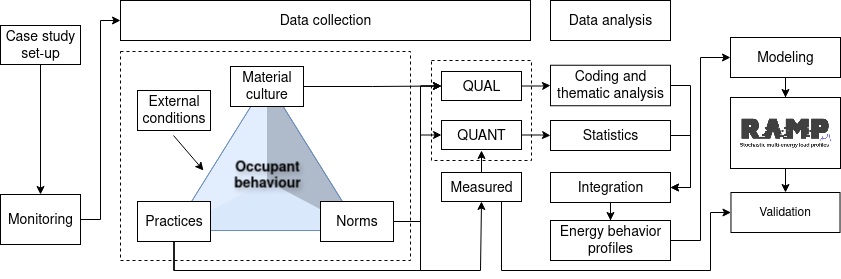
\includegraphics[width=0.8\linewidth]{Figures/EC_method_paper(2).png}
    \caption{Methods flowchart}
    \label{fig:methods}
\end{figure}

\begin{table}[]
\centering
\footnotesize %\normalsize  %\scriptsize % smaller font
\setlength{\tabcolsep}{3pt} % reduce horizontal padding
\renewcommand{\arraystretch}{1.3} % reduce row height
\begin{tabular}{lll}
\hline
\textbf{Dimension} & \textbf{Variables} & \textbf{Indicators} \\ \hline
\multirow{10}{*}{\rotatebox{90}{Material Culture}} &
  \multirow{2}{*}{Energy supply} &
  Technology type \\
 & & Installed capacity \\
 & & Storage Capacity \\
 & Building characteristics & Wall, floor, roof material \\
 & & Building size/rooms \\
 & Appliance ownership & Number of appliances \\
 & & Illumination method \\
 & & Thermal comfort method \\
 & & ICT equipment used \\
 & & Cooking method \\ \hline
\multirow{17}{*}{\rotatebox{90}{Norms}} &
  \multirow{3}{*}{Cultural value of energy} &
  Narratives linking energy use to traditions, identity, or spirituality \\
 & & Expressions of pride or resistance to certain technologies \\
 & & Cultural rituals influencing energy use \\ \cline{2-3} 
 & \multirow{3}{*}{Gender expectations} &
  Roles in appliance use, decision-making, and energy budgeting \\
 & & Frequency of women vs. men performing energy-related tasks \\
 & & Attitudes toward gender participation in energy planning \\ \cline{2-3} 
 & \multirow{4}{*}{Energy aspirations and sufficiency perception} &
  Desired appliances/services vs. current \\
 & & Perceptions of “enough” electricity \\
 & & Satisfaction level with access \\
 & & Aspirations for grid connection/expansion \\ \cline{2-3} 
 & \multirow{4}{*}{Energy conservation and environmental awareness} &
  Awareness of environmental impacts \\
 & & Narratives on saving electricity/waste reduction \\
 & & Self-reported energy conservation practices \\
 & & Frequency of conservation actions \\ \cline{2-3} 
 & Energy sharing &
  Frequency of energy-sharing practices \\
 & & Norms of reciprocity/mutual aid \\
 & & Existence of informal energy-sharing networks \\ \hline
\multirow{10}{*}{\rotatebox{90}{Energy Practices}} &
  \multirow{2}{*}{Daily activities} &
  Main daily energy-related activities \\
 & & Daily activities outside the household \\
 & & Activity timing (morning, evening, seasonal) \\
 & & Productive vs. household activity split \\ \cline{2-3} 
 & Energy use &
  Average daily/weekly usage time \\
 & & Time windows of use \\
 & & Appliance power rating \\
 & & Household energy consumption (kWh) \\
 & & Load profiles based on use and appliance ratings (N) \\
 & & User narratives on appliance importance/constraints \\ \hline
\multirow{9}{*}{\rotatebox{90}{External factors}} &
  \multirow{5}{*}{Socioeconomic conditions} &
  Household size and composition \\
 & & Education levels \\
 & & Income sources \\
 & & Energy expenditure as \% of income \\
 & & Dependency of livelihoods on electricity \\ \cline{2-3} 
 & \multirow{4}{*}{Climatic conditions} &
  Seasonal temperature ranges \\
 & & Daylight hours per season \\
 & & Seasonal accessibility challenges \\
 & & Rainfall patterns and seasonality \\ \hline
\end{tabular}
\caption{Summary of dimensions, variables, and indicators considered in the work within the \ac{EC} framework}
\label{tab:variables}
\end{table}

\subsection{Case Study: An Indigenous Originary Peasant Territory}
\label{sec:case_study}

The study area is located within the Indigenous Originary Peasant Autonomous Territory (TIOC) of Raqaypampa in Bolivia, inhabited by Quechua communities. Officially recognized as the first TIOC in the country on July 12, 2016, Raqaypampa marked a milestone in indigenous self-determination. Its Autonomy Statute was approved by referendum in November 2016, with over 91\% voter support, followed by the first elections of autonomous authorities in June 2017. Grounded in ancestral values and the principle of Sumaq Kawsay (Living Well), the territory is governed through holistic, culturally rooted practices aimed at managing the land in harmony with Pachamama (Mother Earth). Today, Raqaypampa serves as a national reference for community-led governance. The territory encompasses 43 communities across approximately 556 square kilometers, with elevations ranging from 1,600 to 3,300 meters above sea level (See Figure \ref{fig:raq_map}) \cite{oep_estatuto_2016, plan de gestion territorial}. Between 2001 and 2012, the territory experienced a significant population decline, dropping from approximately 10,230 to 7,340 inhabitants. This decrease was largely attributed to permanent migration driven by economic hardship and the absence of basic services. However, according to the most recent national census conducted in 2024, the population has increased slightly, reaching 8,007 inhabitants. The territory’s main economic activities revolve around small-scale agriculture and livestock farming, primarily for household consumption, with surplus production sold in local markets. Key crops include potatoes, maize, wheat, and a variety of vegetables. Livestock such as cattle, goats, and sheep are raised for milk, meat, and wool, contributing both to family subsistence and local trade.



\begin{figure}
    \centering
    \includegraphics[width=0.5\linewidth]{Figures/rap_map.png}
    \caption{Indigenous Originary Peasant Territory of Raqaypampa}
    \label{fig:raq_map}
\end{figure}

This study focuses on an electrification initiative implemented in three communities within the TIOC: Molle Orcko, Ichuqata, Sillar and Tipapampa. These communities are grouped into two zones: Zone A, located in the northwest, which includes Ichuqata, Sillar, and Tipapampa; and Zone B, situated on the eastern side, which comprises Molle Orcko. The initiative is part of a Research for Development project funded by the Belgian institution Académie de Recherche et d’Enseignement Supérieur (ARES). The project involved the distribution of 100 Solar Home Systems (SHS) using a co-financing model, whereby participating families contributed 20\% of the system’s total cost. Starting at the end of 2022, the process was initiated with informational meetings held jointly by researchers, community leaders, and a partnering non-governmental organization (NGO) to present and discuss the project’s objectives. The solar system selection was carried out collaboratively: different SHS options were presented to community members and leaders, with detailed explanations of their technical specifications and associated costs. The final decision was reached through a consensus-based dialogue, reflecting both the communities’ specific energy needs and their financial capacities. A typical household is shown in Figure \ref{fig:typical_household}, featuring the installed Solar Home System.

\begin{figure}
    \centering
    \includegraphics[width=0.5\linewidth]{Figures/household.png}
    \caption{Typical household in Raqaypampa}
    \label{fig:typical_household}
\end{figure}

\begin{table}[]
\centering
\begin{tabular}{ll}
\hline
Component  & Characteristics                                                          \\ \hline
Solar PV   & \begin{tabular}[c]{@{}l@{}}Polycrystalline\\ 20Wp, 12V \end{tabular}       \\ \cline{1-2}
Battery    & \begin{tabular}[c]{@{}l@{}}LiFePO4\\ 12.8V \\ 7000mAh, 89Wh\end{tabular} \\ \cline{1-2}
\multirow{5}{*}{Accessories} & 1 LED light 2W, 200 lm SFL                                               \\
           & 1 LED light 3W, 200 lm SFL                                               \\
           & Phone charging set                                                       \\
           & Metal structure                                                          \\
           & Rechargeable radio                                                       \\ \hline
\end{tabular}
\caption{Characteristics of the Solar Home System acquired by the families in Raqaypampa.}
\label{tab:shs_characteristics}
\end{table}

\subsection{Data collection and analysis}
\label{sec:data_collection_analysis} 
Outline the methods used, such as:

    Prior to establishing the case study, socioeconomic surveys were conducted with the heads of all 100 participating households at the time of SHS deployment in February 2023. The survey collected data on variables included in the External Factors dimension of the Energy Cultures (EC) framework, along with additional indicators characterizing household demographics, livelihoods, and energy access. The full questionnaire is provided in Appendix A. Given the mix of qualitative and quantitative variables, descriptive statistical analyses were performed for both numerical and categorical data to construct a socioeconomic profile of the study population.

    Following SHS deployment, a longitudinal monitoring campaign was implemented to examine patterns of electricity access and use over time. A mixed-methods approach was adopted, combining structured household surveys, semi-structured interviews, focus group discussions, and the installation of household data loggers to monitor energy consumption. These instruments were applied at different stages of the study to capture both baseline conditions and evolving energy practices. Data collection was explicitly structured around the three dimensions of the Energy Cultures framework—material culture, norms, and practices—to provide a comprehensive understanding of the socio-technical context of energy use in the community. A summary table 

    \begin{table}[ht]
\centering
\caption{Overview of data collection methods applied in the Raqaypampa case study.}
\label{tab:data_collection}
\begin{tabular}{p{3cm}p{3cm}p{3cm}p{5cm}}
\toprule
\textbf{Method} & \textbf{Sample size / participants} & \textbf{Timing} & \textbf{Purpose} \\ 
\midrule
Structured household survey I & 100 household heads & February 2023 (baseline) & Collect socioeconomic data, household characteristics, and energy access conditions. \\

Structured household survey II & 53 household members & Nov 2023--December 2025 & Collect self-reported energy practices data. \\

Semi-structured interviews & 25 participants (household heads and key informants) & March--June 2023 & Explore household energy practices, cultural norms, and perceptions of sufficiency. \\

Focus group discussions & 2 groups (10--15 participants each) & April 2023 & Validate survey findings, discuss gender roles, energy-sharing norms, and aspirations. \\

Electricity data loggers & 10 SHS-installed households & Continuous, Apr 2023--Dec 2025 & Record real-time electricity generation and consumption to validate demand modeling. \\ 
\bottomrule
\end{tabular}
\begin{tablenotes}
\small
\item Note: All households are beneficiaries of Solar Home Systems (SHS) deployed in Raqaypampa, Bolivia. Survey instruments and interview guides are provided in Appendix A.
\end{tablenotes}
\end{table}
    
    The methods used to analyze the collected data varied according to the data type, as illustrated in Figure \ref{fig:methods}. Quantitative survey data were analyzed using descriptive statistical techniques implemented in Python, while qualitative data from interviews and focus group discussions were examined through systematic coding and thematic analysis with the open-source tool QualCoder. Measured electricity consumption data from household loggers were processed and analyzed using Python to derive key indicators such as daily load profiles. 
    Qualitative and quantitative data are integrated through a narrative-based approach, in which quantitative energy-use profiles derived from survey responses and measured data are contextualized and explained using qualitative insights from interviews and focus groups. This mixed-methods integration allows for a deeper understanding of not only what energy is used and how much, but also why these patterns emerge, capturing the socio-cultural drivers behind energy behaviors.
    In the final stage, the developed energy-use profiles are incorporated into an electricity demand model to simulate household consumption patterns, and the modeling results are subsequently validated against measured data.

\subsection{Modeling approach: Using RAMP}
\label{sec:modeling}
    In the final stage, the developed energy-use profiles are incorporated into an electricity demand model to simulate household consumption patterns, and the modeling results are subsequently validated against measured data. 
    
\section{Results}
\label{sec:results}

\subsection{Socioeconomic Profile}
\label{sec:raqaypampa}

Household sizes in the targeted communities range from 1 to 12 members, with 66 households located in Zone A and 32 in Zone B. Families are predominantly organized as nuclear (parents and children), extended (including grandparents or other relatives), or large extended households (multiple related families living together). Household heads are most often male (75\%).Household walls are typically constructed from mud bricks, with roofs made of clay tiles, corrugated metal sheets, or straw. Floors are generally earthen. Living spaces are shared for sleeping, while in some cases a separate room is designated for cooking. Additional structures are often built for food storage, known locally as \textit{trofas}, usually made of straw, and for cooking purposes such as ovens. An example of structure distribution is shown in \ref{fig:typical_household}.

Agriculture is the primary economic activity, practiced mainly for subsistence, with surpluses occasionally sold in local markets. Livelihoods remain precarious: at least 60\% of households report earning less than USD 35 per month or having no direct income. Approximately 46\% of households reported that at least one family member engages in temporary migration for work, primarily during the summer months.

Quechua is the dominant language, while Spanish is spoken by a smaller portion of the population, mainly those who have attended school. About half of the households have children currently enrolled in school.

The population relies on natural sources such as springs and rivers for water, as there is no access to potable water infrastructure. In years of drought, water scarcity becomes particularly severe, posing significant challenges for daily life and livelihoods. Cooking is primarily carried out with firewood, and diets are largely based on maize, potatoes, rice, and locally grown vegetables.

The agricultural production cycle is closely tied to the rainy season, as most crops are rain-fed and depend exclusively on rainfall due to the region’s limited access to irrigation water. The cycle typically follows this sequence: soil preparation takes place in August–September, sowing occurs in October–November, cultural practices and crop maintenance extend from October through March, and harvesting takes place in May–June.

\subsection{Energy Practices}
\label{sec:energy_practices}
Findings on self-reported energy practices, actual electricity consumption, and their interplay.
Present interesting indicators to compare real and modeled load curves.

\subsection{Material Culture}
\label{sec:material_culture}
Findings on the role of technologies and infrastructure in shaping energy use.

\subsection{Norms and Perceptions}
\label{sec:norms_perceptions}
Finding on how norms and perceptions shape energy practices. 

\subsection{Interplay of Energy Culture Dimensions and External Influences}
\label{sec:external_influence}


\subsection{Energy Demand Model for Raqaypampa Indigenous Territory}
\label{sec:energy_demand_model}
Results on simulating an energy demand model for all the territory using insights from results in previous sections.

\section{Discussion}
\begin{itemize}
    \item How results are related with the aim of this study?
    \item Comparison of findings to previous studies, highlighting unique contributions, particularly in rural or indigenous contexts.
    \item Implications for Sustainable Energy Planning: Discuss how insights can guide policy and practice, emphasizing the integration of socio-cultural aspects into energy demand modeling. How the model is improved by introducing other aspects? 
    \item Methodological Contributions: Reflect on the mixed-methods approach and its value in data-scarce settings. Is it worth to keep using surveys and traditional methods for data gathering on energy practices? 
\end{itemize}

Edit test

\section{Conclusion}
\label{sec:conslusion}
\begin{itemize}
    \item Context-specific insights from the empirical case study.
    \item Advancements in mixed-methods analysis using the Energy Cultures framework.
    \item Empirical evidence for improving data collection methodologies.
    \item Integration of socio-cultural dimensions into energy demand simulation.
\end{itemize}


%% The Appendices part is started with the command \appendix;
%% appendix sections are then done as normal sections



%% If you have bibdatabase file and want bibtex to generate the
%% bibitems, please use
%%
 \bibliographystyle{elsarticle-num} 
 \bibliography{cas-refs}

%% else use the following coding to input the bibitems directly in the
%% TeX file.

% \begin{thebibliography}{00}

% %% \bibitem{label}
% %% Text of bibliographic item

% \bibitem{}

% \end{thebibliography}
\end{document}
\endinput
%%
%% End of file `elsarticle-template-num.tex'.
